\documentclass[main.tex]{subfiles}
\begin{document}

The design of the package decomposes the quantum walk system's evolution from
equation \eqref{eq:ctqwSystemEvolution}, into several modules: \texttt{State},
for representing initial and final states; \texttt{Operator}, for building the
graph-associated Hamiltonian; \texttt{QuantumWalk}, for combining the operator
and initial state to output the final state; and
\texttt{ProbabilityDistribution}, for converting amplitudes into probabilities.

\begin{figure}[!h]
    \centering
    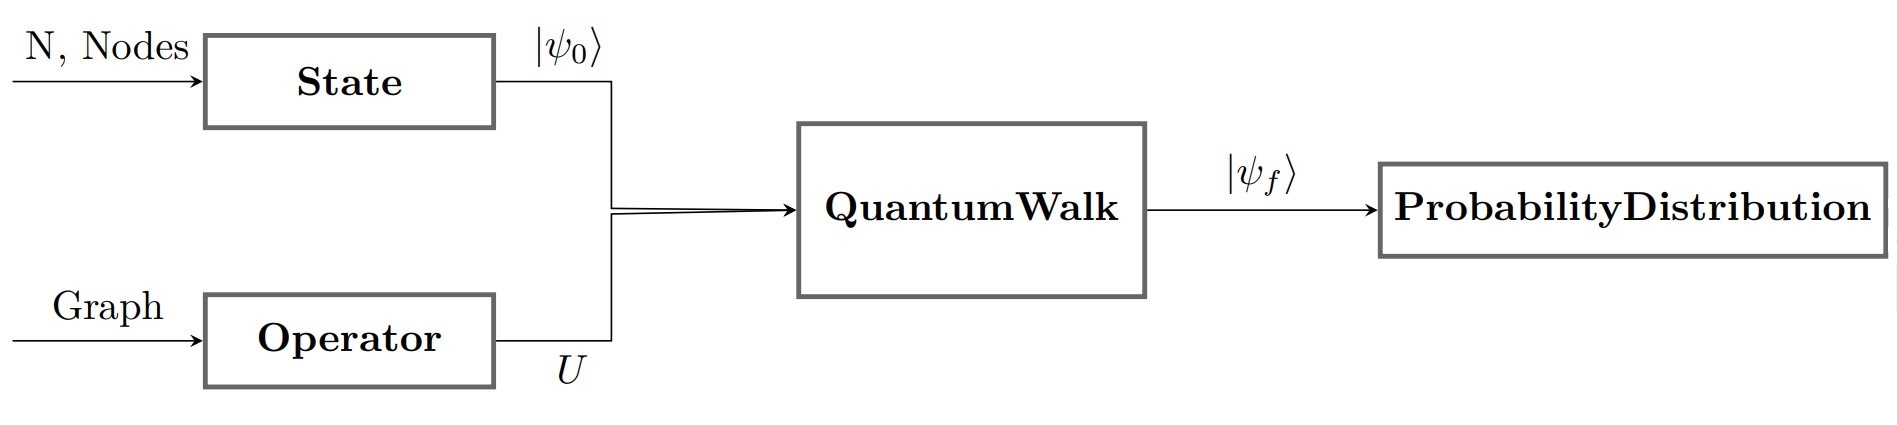
\includegraphics[width=12cm]{qwakDiagram.jpg}
    \caption{Flow-chart of \texttt{QWAK}'s implementation of the CTQW.}
    \label{fig:oriented_line}
\end{figure}

The \texttt{QWAK} class streamlines the package's usage by integrating the
previous components, allowing simplified CTQW simulation and analysis.
Similarly, the stochastic quantum walk is broken down into constituent
entities, later combined in the \texttt{StochasticQWAK} class. In the following
sub-sections, we will go over the individual components of the \texttt{QWAK}
class and their initialization parameters. Note that the following code assumes
\texttt{NumPy} and \texttt{NetworkX} are imported. Documentation is available
on GitHub\footnote{\url{https://jaimepsantos.github.io/QWAK/}}.

\subsubsection{State}

The \texttt{State} class accepts the desired dimension \texttt{n} and creates a
\texttt{ndarray} with corresponding elements. Optional parameters
\texttt{nodeList} and \texttt{customStateList} initialize a uniform
superposition or a custom state, respectively. Default initialization fills
the vector with zeros. If the inputted custom state is not unitary, a
\texttt{NonUnitaryState} exception will be thrown. Similarly, passing a vertex index
greater than the state's dimension will raise a \texttt{StateOutOfBounds}
exception.

For example, creating the uniform superposition of the state
\begin{equation}
    \ket{\psi} = \frac{1}{\sqrt{4}}\left( \ket{0} + \ket{1} +\ket{2} +\ket{3}\right),
\end{equation}
can be done via:

\begin{lstlisting}[style=code]
from qwak.State import State

n = 4
initNodes = [0,1,2,3]
initState = State(n,initNodes)
initState.buildState()
\end{lstlisting}

The \texttt{buildState} function fills the uniform superposition or custom
state arrays. The user can define vertex amplitudes either at
building time, or default to initialization. The \texttt{getStateVec} function
simply returns the array of the state. The remaining available methods are
described in the documentation. 


\subsubsection{Operator and performance}
The \texttt{Operator} class requires a \texttt{NetworkX} graph object with
matching number of vertices, which initializes the internal
\texttt{hamiltonian} attribute. If the \texttt{laplacian} parameter is
\textit{True}, the \texttt{hamiltonian} is built with the Laplacian matrix. The
\texttt{gamma} and \texttt{time} parameters dictate the transition rate and
length of evolution, respectively, and the \texttt{markedElements} parameter
accepts a list of tuples with amplitude-node pairs, modifying the Hamiltonian
to perform a CTQW search.\par

The operator can be constructed via the following procedure:
\begin{lstlisting}[style=code,escapeinside={__}]
from qwak.Operator import Operator 

t = 2
graph = nx.cycle_\textunderscore_graph(n)
operator = Operator(graph)
operator.buildDiagonalOperator(t)
\end{lstlisting}

The \texttt{buildDiagonalOperator} method, crucial for time evolution, posed an
important performance challenge for QWAK. The operator, $U$, was previously
defined in equation \eqref{eq:contSimulUniOp}, where matrix exponentiation is
required. This can be achieved with \texttt{SciPy}'s \texttt{expm} function,
at a significant computational cost. 
\begin{figure}[!h]
    \centering
    \begin{subfigure}[b]{0.49\textwidth}
        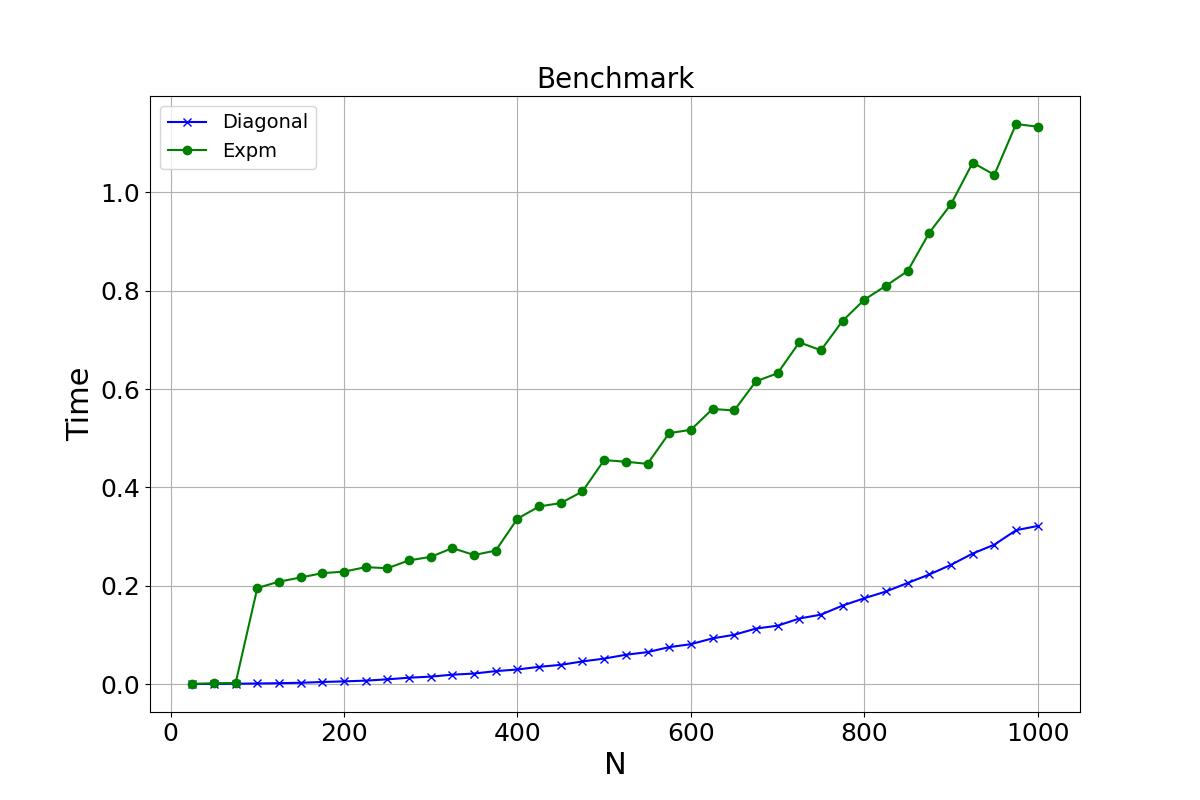
\includegraphics[width=\linewidth]{staticBenchmark_F25_T1000_ST25_TM50_SAMP100.png}
        \caption{Varying the number of vertices.}
        \label{fig:expmVsDiag}
    \end{subfigure}
    \hfill 
    \begin{subfigure}[b]{0.49\textwidth}
        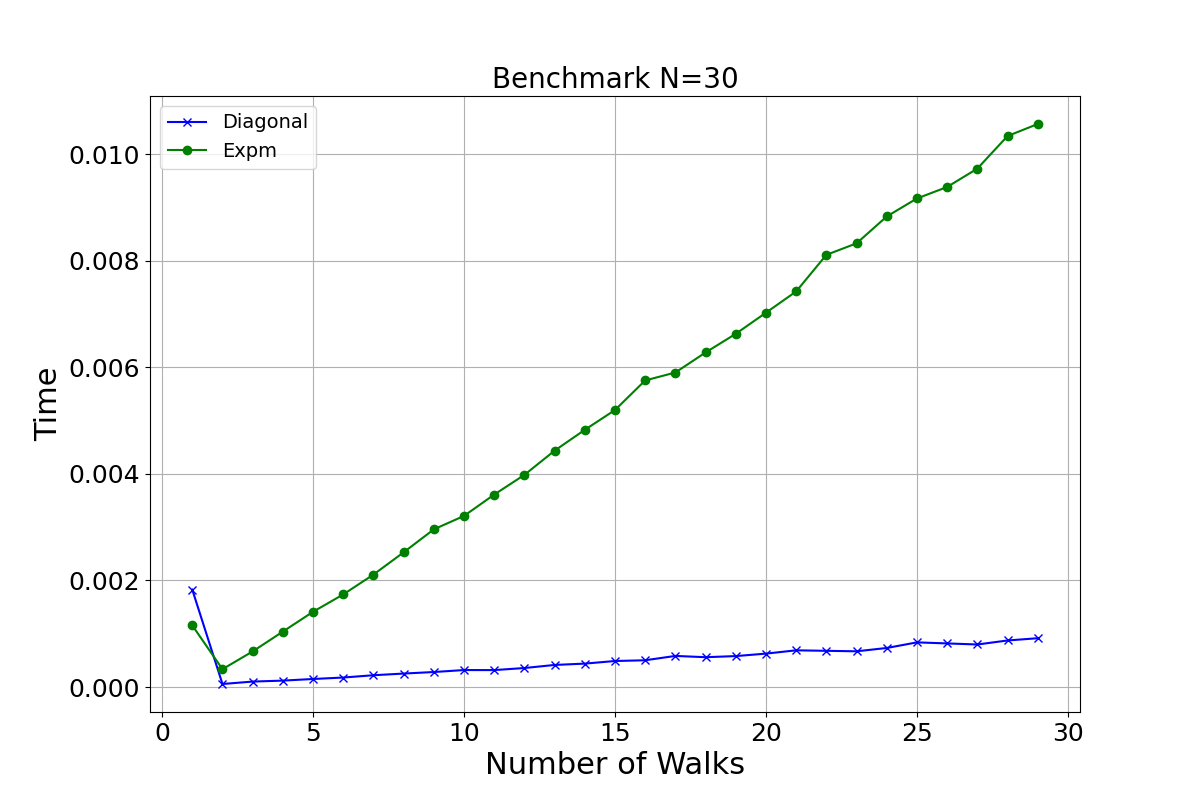
\includegraphics[width=\linewidth]{dynamicBenchmark_WSTART1_WEND30_WST1_SAMP200.png}
        \caption{Varying the number of walks.} 
        \label{fig:expmVsDiagTime}
        \end{subfigure}
   \caption{Comparisons between the execution times of the spectral decomposition and matrix exponential methods.}
   \label{fig:expmVsDiagCombined}
\end{figure}

Alternatively, since we are dealing with diagonalizable matrices, we calculate
the spectral decomposition of $U$
\begin{equation}
    U = Q e^{i\Lambda t} Q^{-1} ,
\end{equation}
where $Q$ is a matrix containing the eigenvectors of the adjacency matrix, and 

\begin{equation}
    \Lambda = \sum_{j} \lambda_j \ket{j}\bra{j},
\end{equation}
is a diagonal operator that encodes the eigenvalues. 

In order to implement this, we use \texttt{NumPy}'s linear algebra methods.
Even though calculating eigenvectors and eigenvalues is relatively costly,
matrix size gets significantly reduced when dealing with hermitian matrices,
resulting in better performance when compared to \texttt{expm} as seen in
figure \ref{fig:expmVsDiag}. The results were obtained by varying the number of
vertices, sampling each experiment $100$ times and plotting the average.\par

The performance advantage of using the \texttt{Operator} implementation becomes
more evident in dynamic evolutions of the CTQW. In a fixed-size graph, the
eigenvectors and eigenvalues remain constant, allowing them to be
pre-calculated during the \texttt{Operator} initialization. This makes
subsequent calls to \texttt{buildDiagonalOperator} more efficient. On the
other hand, the \texttt{expm} method recalculates the matrix exponentiation at
every time step, requiring significant computational resources.\par

Figure \ref{fig:expmVsDiagTime} illustrates this point. It shows that while the
\texttt{eigh} function used in spectral decomposition has a higher initial
computational cost, the subsequent calls follow a much smaller linear
scaling over time compared to \texttt{expm}.\par 

The \texttt{Operator} class also includes a \texttt{checkPST} method, which
identifies perfect state transfer between specific nodes, and calculates
transfer times \cite{coutinho17}.

\subsubsection{QuantumWalk}
We can obtain the final state of the quantum walk evolution by combining the
initial state and operator. This is simplified via the
\texttt{QuantumWalk} class, which takes in the initial state and operator as
parameters. By passing the appropriate values, we can easily obtain the
final state:

\begin{lstlisting}[style=code,escapeinside={__}]
from qwak.QuantumWalk import QuantumWalk 

quantumWalk = QuantumWalk(initState,operator)
quantumWalk.buildWalk()
finalState = quantumWalk.getFinalState()
\end{lstlisting}

The \texttt{buildWalk} method multiplies the operator matrix with the state
array, setting the \texttt{finalState} attribute to the resulting amplitudes.
The \texttt{State} object can be accessed via \texttt{getFinalState}, and the
associated \texttt{ndarray} with \texttt{getStateVec}. The class also offers
transport property calculation methods, such as transport efficiency
\cite{razzoli21}, and inverse participation ratio \cite{buarqueAperiodic19}.

\subsubsection{ProbabilityDistribution}
This class takes a \texttt{State} object, generally a final state, and converts
amplitudes into probabilities according to the Born rule. The \texttt{probVec}
attribute is initialized with a zero-filled \texttt{ndarray}, and can be
constructed using the previous state as follows:

\begin{lstlisting}[style=code,escapeinside={__}]
from qwak.ProbabilityDistribution import ProbabilityDistribution

probDist = ProbabilityDistribution(finalState)
probDist.buildProbDist()
\end{lstlisting}

The \texttt{buildProbDist} is responsible for multiplying each element of the
\texttt{finalState} array by its conjugate. The desired state can be altered at
build time. Another notable method computes the survival probability
\cite{buarqueAperiodic19}, accessible through the \texttt{survivalProb} method.

\subsubsection{QWAK Class}

The \texttt{QWAK} class coordinates all of the previous components, providing a
quick and convenient way for simulation.  It's main purpose is to remove the
need to manually define each object and to simplify the overall workflow. Since
the parameters for this class have been previously discussed, we will move
forward with a practical example:

\begin{lstlisting}[style=code,escapeinside={__}]
from qwak.qwak import QWAK

t = 40
n = 200
graph = nx.circular_\textunderscore_ladder_\textunderscore_graph(n)
initSt = [(n // 2,1/np.sqrt(2)),(n // 2 + 1,1/np.sqrt(2))]
qwController = QWAK(graph,customStateList=initSt)
qwController.runWalk(t, initNodes)
plt.plot(qwController.getProbVec())
\end{lstlisting}

Figure \ref{fig:probDistCircLadder} depicts the distribution of a circular
ladder graph formed from the Cartesian product of two cycle graphs, resulting
in two distinct waveforms. The \texttt{NetworkX} function creates two connected
cycles with size $n$, totaling $2n$ nodes. The example also demonstrates the
\texttt{customStateList} parameter, which throws an exception if the sum of the
amplitudes is not equal to $1$.\par

\begin{figure}[!h]
\centering
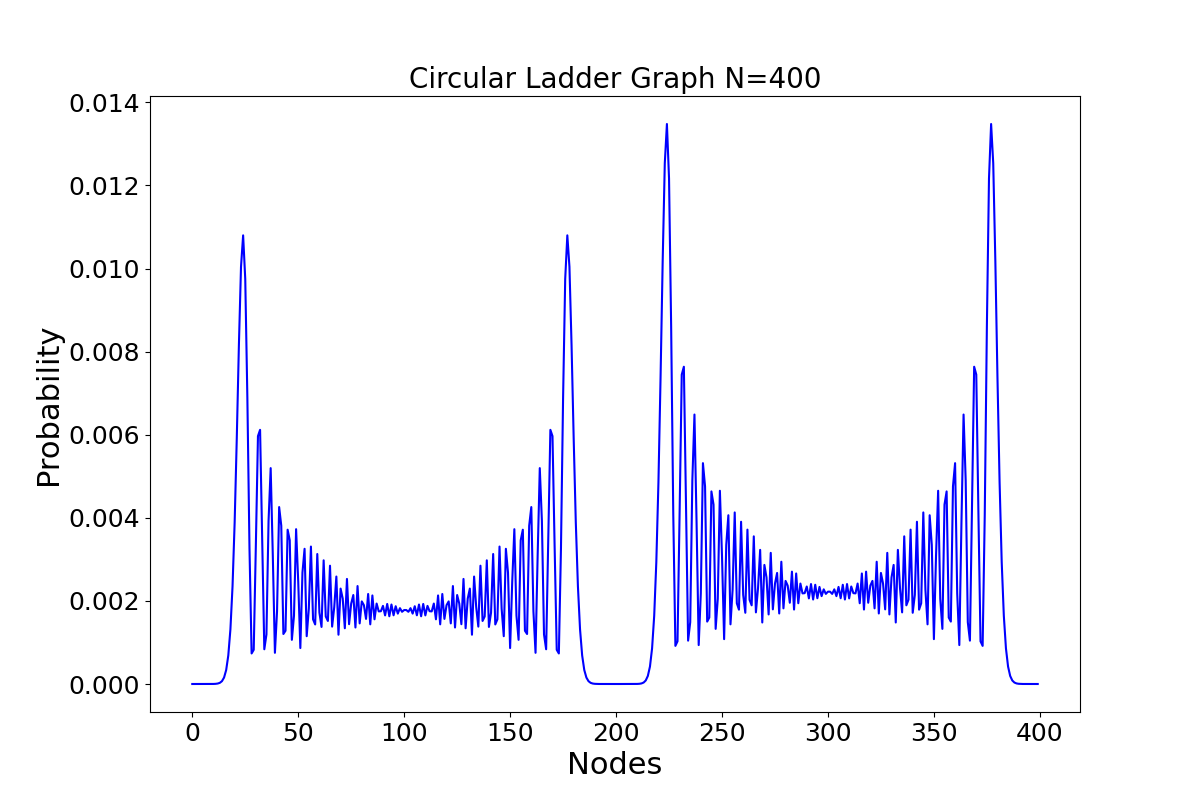
\includegraphics[scale=\mysinglefigurescale]{circularLadderDynamics_N400_TMAX40.png}
\caption{Probability distribution for the CTQW on a
circular ladder graph of size $N=400$, at $t=40$, with initial condition
$\ket{\psi(0)}=\frac{\ket{100}+\ket{101}}{\sqrt{2}}$ and $\gamma=1$.}
\label{fig:probDistCircLadder}
\end{figure}

During initialization, the \texttt{QWAK} object creates attributes by calling
the previously defined classes based on the given parameters. The
\texttt{runWalk} method incorporates the aforementioned build methods and
handles any exceptions raised. Users can modify initialization values through
the optional parameters. Additional examples, including transport property
calculation and stochastic quantum walk simulation, can be found in the
\texttt{GitHub} repository.

\end{document}
